\documentclass[preprint,12pt,authoryear]{elsarticle}

\usepackage{booktabs}
\usepackage{amsmath}
\usepackage{hyperref}
\hypersetup{hypertexnames=false}
\usepackage{tikz}
\usepackage{pgfplots}
\pgfplotsset{compat=1.18}
\usetikzlibrary{positioning}
\emergencystretch=3em

\journal{Ecological Informatics}

\begin{document}

\begin{frontmatter}

\title{Convention-aware and reproducibly validated biodiversity computation for ecological informatics}

\author[inst1]{Matthew Roughan}
\affiliation[inst1]{
  organization={Affiliation to be supplied},
  city={},
  country={}
}

\begin{abstract}
Biodiversity indices are central to ecological informatics, microbial ecology,
conservation assessment, and ecosystem monitoring, yet many commonly used
indices are convention-sensitive.  Names such as Simpson, Shannon, Jaccard,
and Sorensen can refer to different transformations, logarithm bases, input
types, or similarity-versus-dissimilarity conventions across software
ecosystems.  These differences create a reproducibility problem for
data-intensive ecological workflows, where alpha-diversity summaries,
estimator diagnostics, and pairwise dissimilarity matrices are often combined
in downstream analyses.  We present \texttt{DiversityAndDissimilarity.jl}, a Julia
package designed as an ecoinformatics infrastructure layer for reproducible
diversity computation.  Its three core contributions are: (1) a
convention-aware metadata and trait system that exposes index families, input
modes, output modes, ranges, aliases, and metric properties as machine-readable
data; (2) an executable validation and benchmark corpus that links
formula-level reference cases, cross-package migration checks, documentation,
figures, and performance reports; and (3) workflow audit reports that combine
alpha-diversity summaries, coverage diagnostics, pairwise distances, and
bootstrap uncertainty intervals.  The package treats diversity and
similarity indices as related computational objects because they share data
orientation, normalization, incidence, abundance, and labeling assumptions.
Benchmarks against R and Python demonstrate that reproducibility-oriented
metadata can coexist with optimized matrix kernels.  The result is not only a
library of biodiversity indices, but a framework for making biodiversity
calculations inspectable, testable, and portable across ecological data
workflows.
\end{abstract}

\begin{highlights}
\item Biodiversity index conventions are exposed as machine-readable metadata.
\item Diversity and similarity indices are integrated in one auditable workflow.
\item Executable reference cases link formulas, tests, documentation, and benchmarks.
\item Workflow audits combine coverage diagnostics and bootstrap uncertainty reports.
\item Warmed cross-language benchmarks compare Julia, R \texttt{vegan}, and Python.
\end{highlights}

\begin{keyword}
biodiversity informatics \sep ecological informatics \sep diversity indices
\sep beta diversity \sep reproducible research \sep Julia
\end{keyword}

\end{frontmatter}

\section{Introduction}

Ecological informatics is concerned with the computational representation,
analysis, and reuse of ecological data.  Biodiversity measurement is one of
its recurring building blocks: richness, Shannon entropy, Simpson-family
measures, Hill numbers, and pairwise similarities or dissimilarities are used
to summarize communities, compare sites, diagnose sampling effort, and support
ordination, clustering, monitoring, and conservation decisions
\citep{hill1973diversity,jost2006entropy,chao1984nonparametric,
whittaker1960vegetation,legendre2012numerical}.  As ecological datasets grow
larger and more heterogeneous, these calculations increasingly occur inside
automated workflows rather than as isolated hand calculations.

That automation exposes a persistent problem: biodiversity indices are not
only mathematical formulas, but also software conventions.  ``Simpson
diversity'' can mean concentration, its complement, or its reciprocal.
Shannon entropy can be reported in nats, bits, or as an effective number after
exponentiation.  Jaccard and Sorensen--Dice can refer to binary incidence
similarities, abundance-sensitive variants, or their distance complements.
These differences are often well documented within individual software
ecosystems, but documentation written as prose is easy to miss when results
are passed between R, Python, Julia, spreadsheets, notebooks, reports, and
data repositories.

The consequence is an ecoinformatics reproducibility problem.  A numerical
value may be correct within one package and misleading when interpreted under
another package's naming convention.  A distance matrix may be generated from
relative abundances in one workflow and incidence data in another.  An index
may be treated as a metric by downstream algorithms even when it does not
satisfy metric assumptions.  These problems are subtle because they need not
produce errors: they produce plausible but differently defined results.

We present \texttt{DiversityAndDissimilarity.jl}, a Julia package designed to make
these conventions explicit and executable.  The package provides scalar,
matrix, and table-oriented biodiversity calculations, but its main novelty is
not the existence of another index library.  Instead, the package treats
index definitions, cross-package conventions, validation examples, benchmark
results, and workflow diagnostics as connected computational artifacts.
This orientation aligns with the broader goals of reproducible and reusable
research software \citep{peng2011reproducible,wilkinson2016fair}.

The paper makes three contributions.  First, we introduce a convention-aware
metadata and trait layer for diversity and similarity indices.  Index objects
report their family, input mode, output mode, range, aliases, metric status,
and availability of optimized matrix kernels.  Second, we introduce an
executable validation and benchmark corpus.  Formula-level reference cases,
cross-package migration checks, documentation examples, figures, and
benchmark tables are generated from the same package-controlled sources.
Third, we introduce workflow audit reports that keep estimator diagnostics,
coverage checks, pairwise matrices, and bootstrap uncertainty intervals tied
to the same labels and input data.  The paper is therefore framed around
reproducible biodiversity computation rather than around a static software
description.

\section{Background and Motivation}

\subsection{Convention-sensitive biodiversity computation}

The need for explicit conventions is clearest in the Simpson family.  The
concentration
\[
  \lambda = \sum_i p_i^2
\]
is a dominance measure: larger values indicate greater dominance by common
classes.  The Gini--Simpson form, \(1-\lambda\), reverses that interpretation.
The inverse Simpson form, \(1/\lambda\), reports an effective diversity.  All
three are legitimate, but a plot, table, or downstream model that labels all
of them as ``Simpson'' is underspecified.

Similar ambiguity occurs for entropy and pairwise indices.  Shannon entropy
depends on the logarithm base, and Hill-number transformations change the
scale from entropy to effective diversity \citep{hill1973diversity,
jost2006entropy}.  Jaccard and Sorensen--Dice indices depend on whether input
data are interpreted as incidence or abundance.  Bray--Curtis, Hellinger, and
related dissimilarities require choices about normalization and matrix
orientation.  These choices matter for ecological interpretation and for
algorithmic compatibility.

\subsection{Why diversity and similarity indices belong together}

Software often separates alpha-diversity functions from similarity or
dissimilarity functions.  The distinction is ecologically meaningful:
single-sample richness and entropy summarize within-sample diversity, whereas
Bray--Curtis, Jaccard, Sorensen--Dice, and Hellinger comparisons describe
between-sample relationships.  In data analysis, however, they are usually
computed from the same sample-by-taxon matrix and reported together.  A
monitoring workflow may calculate richness and Shannon entropy per site, then
construct a Bray--Curtis matrix for ordination or clustering.  A microbiome
workflow may report alpha-diversity summaries beside incidence-based
beta-diversity comparisons.

Putting these calculations in one package has three advantages for ecological
informatics.  First, it makes shared assumptions visible.  Incidence Jaccard
and richness both depend on non-zero support; Bray--Curtis and Simpson-family
indices are abundance-sensitive; Hellinger distances depend on normalized
profiles.  Second, it protects workflow integrity.  Labels, sample ordering,
matrix orientation, and distance-versus-similarity conventions are tracked in
one computational setting rather than reconstructed manually.  Third, it makes
extension systematic.  A new index can participate in scalar calculations,
matrix kernels, reference validation, documentation, and benchmark reporting
through the same dispatch and metadata interface.

\section{Software Design}

\subsection{Convention-aware index metadata}

\texttt{DiversityAndDissimilarity.jl} represents indices as small dispatchable objects
and exposes their interpretation through trait-like metadata functions.
For each supported index, the package records the index family, expected input
mode, output mode, numerical range, metric status, aliases, convention notes,
and whether a specialized matrix kernel is available.  Figure
\ref{fig:framework} summarizes the design.

\begin{figure}[t]
\centering
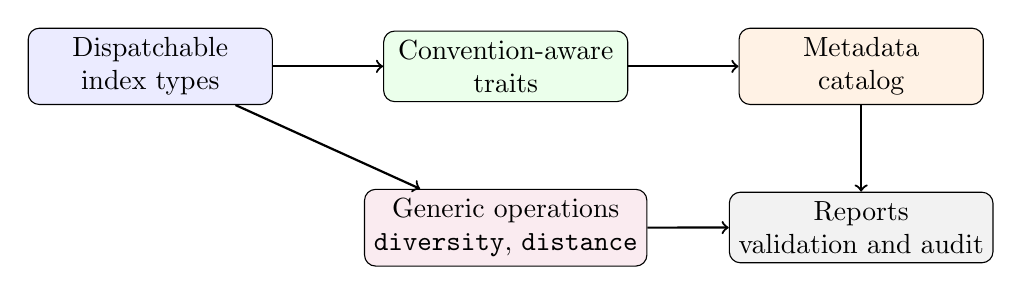
\begin{tikzpicture}[
  node distance=1.1cm and 1.4cm,
  box/.style={draw, rounded corners, align=center, minimum width=3.1cm, minimum height=0.85cm},
  arrow/.style={->, thick}
]
\node[box, fill=blue!8] (types) {Dispatchable\\index types};
\node[box, fill=green!8, right=of types] (traits) {Convention-aware\\traits};
\node[box, fill=orange!10, right=of traits] (metadata) {Metadata\\catalog};
\node[box, fill=purple!8, below=of traits] (ops) {Generic operations\\\texttt{diversity}, \texttt{distance}};
\node[box, fill=gray!10, below=of metadata] (audit) {Reports\\validation and audit};
\draw[arrow] (types) -- (traits);
\draw[arrow] (traits) -- (metadata);
\draw[arrow] (types) -- (ops);
\draw[arrow] (metadata) -- (audit);
\draw[arrow] (ops) -- (audit);
\end{tikzpicture}
\caption{The package separates index identity, convention metadata, and numerical evaluation. This supports generic workflows while keeping naming and output conventions explicit.}
\label{fig:framework}
\end{figure}


For example, \texttt{Simpson()} is defined as concentration, while
\texttt{GiniSimpson()} is the complement used by common R workflows; this
matches the \texttt{simpson} option in \texttt{vegan::diversity}
\citep{oksanen2022vegan}.  The metadata layer makes that distinction
available to users and to programs.
A report generator can label an output as a concentration, a similarity, or a
dissimilarity.  A workflow audit can warn when an index is not a metric.  A
documentation page can group indices by input mode rather than by informal
name.

The design is intentionally lightweight.  Metadata functions return ordinary
Julia values such as symbols, named tuples, and strings.  This avoids a heavy
ontology while still making convention information inspectable and
machine-readable.  Multiple dispatch selects calculations; metadata functions
describe interpretation.  The result is a separation between the numerical
method and the semantic commitments that travel with it.

\subsection{Executable validation corpus}

The second software-design component is an executable validation corpus.
The package exposes formula-level and cross-package reference cases through
the public API.  These cases include small examples for Shannon entropy,
Simpson-family transformations, Bray--Curtis dissimilarity, incidence
Jaccard, Sorensen--Dice, and Pielou evenness.  Each reference case has an
expected value, tolerance, and convention label.  Figure \ref{fig:validation}
shows how these cases connect tests, documentation, benchmarks, and manuscript
artifacts.

\begin{figure}[t]
\centering
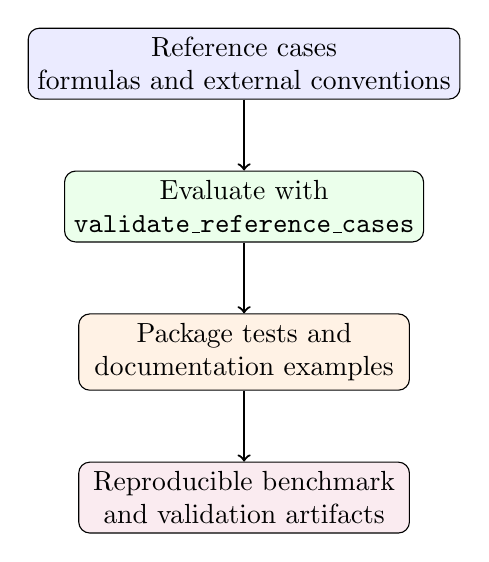
\begin{tikzpicture}[
  node distance=0.9cm,
  box/.style={draw, rounded corners, align=center, minimum width=4.2cm, minimum height=0.75cm},
  arrow/.style={->, thick}
]
\node[box, fill=blue!8] (cases) {Reference cases\\formulas and external conventions};
\node[box, fill=green!8, below=of cases] (evaluate) {Evaluate with\\\texttt{validate\_reference\_cases}};
\node[box, fill=orange!10, below=of evaluate] (tests) {Package tests and\\documentation examples};
\node[box, fill=purple!8, below=of tests] (paper) {Reproducible benchmark\\and validation artifacts};
\draw[arrow] (cases) -- (evaluate);
\draw[arrow] (evaluate) -- (tests);
\draw[arrow] (tests) -- (paper);
\end{tikzpicture}
\caption{The validation corpus makes convention choices executable and visible in tests, documentation, and paper artifacts.}
\label{fig:validation}
\end{figure}


This corpus serves a different role from ordinary unit tests.  Unit tests
guard implementation details; reference cases communicate meaning.  They are
small enough to inspect by hand and structured enough to evaluate
automatically.  They also support migration from established tools.  A user
moving from \texttt{vegan}, for example, can verify that Shannon, Gini--Simpson,
inverse Simpson, and Bray--Curtis examples match the intended R conventions
before translating a larger workflow.

\subsection{Workflow helpers and audit reports}

The package includes workflow-level helpers because reproducibility failures
often occur between calculations rather than inside a single formula.  The
\texttt{estimator\_report} function reports observed richness, singleton and
doubleton counts, sample coverage, Shannon estimator results, effective
diversities, and warnings.  This makes estimator assumptions visible when
sample size and unseen taxa may influence interpretation
\citep{chao2003nonparametric}.
Low-sample corrections for entropy and information divergences are grounded in
the same sampling problem.  The plugin entropy estimator has a systematic
finite-sample bias \citep{paninski2003entropy}; Miller--Madow-style corrections
address the leading entropy-term bias, whereas pseudocount and shrinkage
estimators trade bias for finite estimates when categories are sparse.  For
unseen categories, Good--Turing coverage estimates \citep{good1953population}
and later unseen-estimation work \citep{valiant2017estimating} motivate
explicit unseen-mass corrections.  Minimax results for large alphabets
\citep{jiao2015minimax,wu2016minimax} show why naive plugin estimators can be
fragile when support size is comparable with sample size.  Bayesian entropy
estimators such as the NSB prior \citep{nemenman2002entropy} provide another
route to low-sample information-functional estimation, and motivate exposing
Bayesian smoothing options for KL and Jensen--Shannon-style divergences.

The \texttt{diversity\_audit} function combines alpha summaries, estimator
diagnostics, labeled pairwise matrices, and warnings about potentially
problematic inputs.  It is designed as an early-stage diagnostic for ecological
data analysis: users can check row totals, coverage, labels, and
convention-sensitive distance choices before moving to ordination, clustering,
or modelling.

The \texttt{uncertainty\_audit} function extends this workflow layer by
summarizing bootstrap uncertainty for Shannon entropy and effective Shannon
diversity.  It reports per-sample estimates, standard errors, percentile
intervals, sample coverage, and labels.  The goal is not to replace a full
model-based analysis of uncertainty, but to make early uncertainty diagnostics
available at the same stage as convention and coverage checks.  This is useful
in ecological informatics workflows because uncertainty is often lost when
alpha summaries and distance matrices are exported as separate tables.

\section{Reproducibility and Benchmark Methods}

Reproducibility is addressed at three levels: definitions, computations, and
performance claims.  Definition reproducibility is provided by the metadata
layer: each index object carries convention information that can be inspected
where the calculation is made.  Computational reproducibility is provided by
the validation corpus: reference cases can be run by users, test suites,
documentation builds, and manuscript-generation scripts.  Performance
reproducibility is provided by benchmark scripts that generate tabular
results, figures, and environment metadata.

The benchmark corpus compares \texttt{DiversityAndDissimilarity.jl} with R
\texttt{vegan} and Python/NumPy/SciPy on simulated community matrices.  The
benchmarks include richness, alpha-diversity summaries, Bray--Curtis distance
matrices, Hellinger distance matrices, and incidence Jaccard matrices.  The
scripts record hardware and runtime metadata, including processor, operating
system, Julia version, Julia thread count, Python interpreter, and R stack
where available.  Julia functions are warmed before timing so that reported
values describe steady-state execution rather than just-in-time compilation.
Very fast operations are timed using repeated inner calls to avoid
zero-valued or timer-resolution-limited measurements.

The benchmarks are intentionally workflow-level comparisons.  They include
the costs of normalization, matrix traversal, allocation, and pairwise scaling
because these costs are visible to users in ecological data analysis.  The
results are not claims about universal language performance; they are
reproducible checks on the package's implementation choices for common
ecoinformatics tasks.

The repository also includes a cross-package validation data directory.  It
contains a simulated sample-by-taxon community matrix, hand-checkable paired
vectors, and a manifest mapping validation tasks to equivalent
\texttt{DiversityAndDissimilarity.jl}, R \texttt{vegan}, SciPy, and scikit-bio-style
calls.  These files are intended as a seed for a larger biodiversity software
concordance suite.  They separate the validation data from the package-specific
function calls and from the convention being tested.

\section{Results}

\subsection{Reproducible convention checks}

The executable reference corpus currently validates scalar alpha-diversity
indices and pairwise similarity/dissimilarity indices against formula-level
and cross-package expectations.  Its main practical result is that
conventions become testable objects.  A documentation statement such as
``\texttt{GiniSimpson()} follows the R \texttt{vegan} Simpson convention'' is
backed by an executable case rather than only by prose.  Optimized kernels
and table-oriented helpers can therefore be checked against the same small
reference cases used to explain the package to users.

\subsection{Benchmark results}

Selected warmed per-call benchmark results are shown in Table
\ref{tab:benchmarks}.  They demonstrate that the additional metadata and
validation machinery does not prevent efficient matrix implementations.  In
particular, incidence Jaccard distance matrices benefit from packed
\texttt{UInt64} bitsets, reducing pairwise comparisons to word-wise
intersections, unions, and population counts.

\begin{table}[t]
\centering
\caption{Selected warmed, per-call benchmark results on Intel(R) Core(TM) Ultra 9 285K with Julia 1.12.6 using 1 Julia thread(s). Times in seconds. \emph{Julia (safe)} validates on every call (the default user experience); \emph{Julia (pre)} calls \texttt{validate} once before the timing loop, matching the Python and R calling convention. Dashes indicate no direct equivalent in that stack.}
\label{tab:benchmarks}
\small
\resizebox{\textwidth}{!}{%
\begin{tabular}{llrrrr}
\toprule
Scenario & Task & Julia (safe) & Julia (pre) & Python & R/\texttt{vegan}\\
\midrule
default & richness & $5.8 \times 10^{-5}$ & $5.87 \times 10^{-6}$ & $2.88 \times 10^{-5}$ & $4 \times 10^{-4}$\\
default & Shannon entropy & $2.99 \times 10^{-4}$ & $2.45 \times 10^{-4}$ & $7.91 \times 10^{-4}$ & $1.75 \times 10^{-3}$\\
default & Bray--Curtis matrix & $5 \times 10^{-3}$ & $4.94 \times 10^{-3}$ & $6.06 \times 10^{-3}$ & $8.15 \times 10^{-3}$\\
default & Jaccard matrix & $3.33 \times 10^{-4}$ & $2.56 \times 10^{-4}$ & $1.45 \times 10^{-2}$ & $9.4 \times 10^{-3}$\\
default & Hellinger matrix & $5.25 \times 10^{-3}$ & $5.16 \times 10^{-3}$ & $8.31 \times 10^{-2}$ & ---\\
\midrule
large & Bray--Curtis matrix & $7.31 \times 10^{-2}$ & $7.15 \times 10^{-2}$ & $8.37 \times 10^{-2}$ & $1.29 \times 10^{-1}$\\
large & Jaccard matrix & $3.39 \times 10^{-3}$ & $2.87 \times 10^{-3}$ & $1.98 \times 10^{-1}$ & $1.38 \times 10^{-1}$\\
\bottomrule
\end{tabular}
}
\end{table}


\begin{figure}[t]
\centering
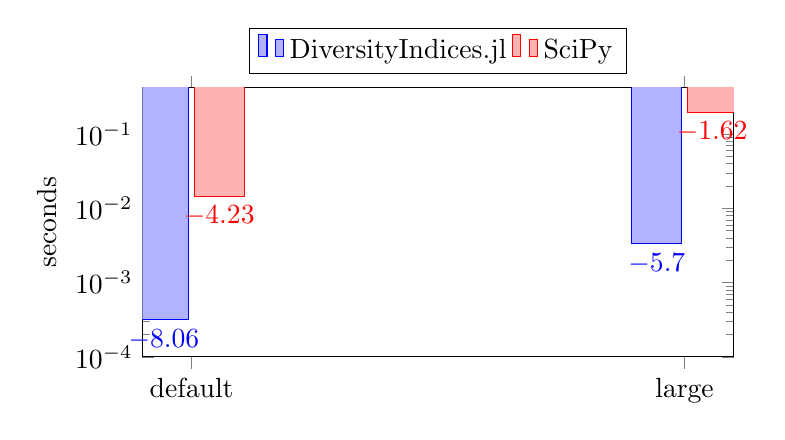
\begin{tikzpicture}
\begin{axis}[
  ybar,
  bar width=18pt,
  ymode=log,
  ylabel={seconds},
  symbolic x coords={default,large},
  xtick=data,
  legend style={at={(0.5,1.05)},anchor=south,legend columns=2},
  width=0.75\linewidth,
  height=5cm,
  ymin=0.0001,
  nodes near coords,
  nodes near coords align={vertical},
]
\addplot coordinates {(default,0.000315) (large,0.00336)};
\addplot coordinates {(default,0.0145) (large,0.197)};
\legend{DiversityIndices.jl,SciPy}
\end{axis}
\end{tikzpicture}
\caption{Selected Jaccard distance matrix timings after bitset incidence encoding. The benchmark is workflow-level and hardware-dependent, but illustrates the algorithmic benefit of packed incidence representation.}
\label{fig:jaccard}
\end{figure}


The benchmark results also show why reproducible performance reporting is
important.  Some tasks are dominated by simple reductions, some by memory
access patterns, and others by pairwise matrix construction.  Profiling and
benchmarking guided targeted implementation improvements, including
column-major matrix traversal and bitset incidence kernels, while the
reference corpus checked that optimized methods preserved the intended
conventions.

\subsection{Workflow case study with uncertainty audit}

We added a simulated forest-gradient workflow case study based on the
cross-package validation matrix.  The case study reads a sample-by-taxon
matrix with habitat and gradient metadata, runs \texttt{diversity\_audit} for
alpha summaries and a labeled Bray--Curtis distance matrix, and then runs
\texttt{uncertainty\_audit} to bootstrap Shannon entropy and effective
diversity for each plot.  Table \ref{tab:case-study} shows the generated
audit table.

\begin{table}[t]
\centering
\caption{Selected workflow case-study audit results. Shannon values are bootstrap estimates with percentile intervals from \texttt{uncertainty\_audit}.}
\label{tab:case-study}
\small
\resizebox{\textwidth}{!}{%
\begin{tabular}{llrlll}
\toprule
Site & Habitat & Richness & Coverage & Shannon H & Effective D\\
\midrule
plot\_A & forest & 7 & 0.979 & 2.31 [1.85, 2.509] & 4.96 [3.704, 5.6]\\
plot\_B & forest & 8 & 0.912 & 2.443 [1.795, 2.657] & 5.438 [3.659, 6.147]\\
plot\_C & forest & 8 & 0.923 & 2.686 [2.054, 2.81] & 6.437 [4.183, 7.021]\\
plot\_D & forest & 7 & 0.923 & 2.439 [1.834, 2.599] & 5.423 [3.557, 6.201]\\
plot\_E & wetland & 8 & 0.939 & 2.575 [2.017, 2.747] & 5.959 [3.952, 6.537]\\
plot\_F & wetland & 8 & 0.951 & 2.504 [2.007, 2.712] & 5.671 [3.925, 6.469]\\
plot\_G & grassland & 8 & 0.909 & 2.457 [1.902, 2.634] & 5.491 [3.778, 6.454]\\
plot\_H & grassland & 7 & 0.941 & 2.352 [1.847, 2.557] & 5.107 [3.622, 5.714]\\
\bottomrule
\end{tabular}
}
\end{table}


This example illustrates the package's third contribution: uncertainty,
coverage, labels, and pairwise comparisons remain part of one reproducible
workflow.  The case study report is generated by a repository script, and the
LaTeX table used here is produced from the same script.  As with the benchmark
section, the manuscript artifact is downstream of executable package
artifacts rather than manually copied results.

\section{Discussion}

\subsection{Contribution to ecological informatics}

\texttt{DiversityAndDissimilarity.jl} contributes to ecological informatics by treating
biodiversity calculation as an information-management problem as well as a
numerical one.  The package does not merely compute indices; it records and
exposes the interpretive context needed to reuse those computations.  This is
important for data-intensive ecology, where biodiversity summaries are
increasingly embedded in automated pipelines, dashboards, teaching materials,
benchmark studies, and reproducible research compendia.

The integration of diversity and similarity indices is central to this
contribution.  Alpha-diversity and beta-diversity calculations differ
ecologically, but they share computational assumptions about matrix
orientation, incidence, abundance, normalization, labels, and output mode.
Placing them behind a shared metadata and validation interface helps users
maintain coherence across the steps of a biodiversity workflow.

The workflow audit contribution extends the same idea to uncertainty.  In
many ecological analyses, point estimates are computed early and uncertainty
is considered later, often after labels and conventions have already been
transformed into intermediate files.  By making bootstrap summaries, coverage
diagnostics, and pairwise matrices available together, the package encourages
users to identify low-coverage or high-uncertainty samples before committing
to downstream analyses.

\subsection{Limitations}

The current package is focused on taxonomic diversity and common
similarity/dissimilarity indices.  It does not yet provide a comprehensive
framework for phylogenetic diversity, functional diversity, rarefaction
curves, uncertainty propagation across full workflows, sparse matrix kernels,
or threaded large-scale distance calculations.  The validation corpus is also
deliberately small: it emphasizes inspectable convention examples rather than
exhaustive coverage of all possible input types.

These limitations are useful because they identify the next layer of
ecoinformatics value.  The same metadata design could be extended to record
phylogenetic trees, trait spaces, abundance transformations, compositional
data assumptions, and estimator uncertainty.  The same validation corpus
could be expanded into a community-maintained benchmark and convention suite
for biodiversity software.

\subsection{Future work}

Future work should prioritize features that increase scientific value rather
than simply increasing the number of indices.  High-value extensions include
sparse and threaded matrix kernels for large monitoring datasets, uncertainty
and bootstrap reports for estimator workflows, first-class support for
phylogenetic and functional diversity, and a richer cross-package validation
suite covering R, Python, and Julia biodiversity tools.  These additions would
make the package a stronger platform for computational biodiversity research
and a more compelling contribution to ecological informatics.

\section{Conclusion}

Reproducible biodiversity analysis requires more than correct formulas.
It requires explicit conventions, executable validation, portable workflow
diagnostics, and performance reports that can be regenerated as software and
hardware change.  \texttt{DiversityAndDissimilarity.jl} provides these elements through
a convention-aware metadata layer and an executable validation and benchmark
corpus.  By treating diversity and similarity indices as related computational
objects, the package supports coherent, auditable biodiversity workflows for
ecological informatics.

\section*{Data and code availability}

The software, validation cases, benchmark scripts, documentation, manuscript
source, validation datasets, workflow case-study scripts, and
figure-generation artifacts are available in the \texttt{DiversityAndDissimilarity.jl}
source repository.  Benchmark tables, case-study tables, and figures used in
this manuscript are generated from repository scripts rather than hand-entered
values.

\section*{Declaration of competing interest}

The author declares no competing interests.

\section*{Funding}

No specific funding statement has been supplied for this draft.

\section*{CRediT authorship contribution statement}

Matthew Roughan: Conceptualization, Software, Methodology, Validation,
Writing -- original draft, Writing -- review and editing.

\bibliographystyle{elsarticle-harv}
\bibliography{references}

\end{document}
